%============================================================
%  Capitolo 10 – Autoencoder
%============================================================
\chapter{Autoencoder}
\label{ch:autoencoders}

Gli autoencoder sono reti neurali addestrate a riprodurre il proprio input
all'uscita. L'obiettivo apparente è banale ($h_\theta(\mathbf{x}) \approx
\mathbf{x}$), ma l'interesse non risiede nell'output bensì nella
\textbf{rappresentazione interna} appresa durante il processo. Imponendo
opportuni vincoli sul collo di bottiglia centrale, la rete è costretta a
estrarre una rappresentazione compatta e informativa dei dati,
utile per compressione, riduzione dimensionale, generazione e
pre-addestramento non supervisionato \citep{bishop2024}.

%------------------------------------------------------------
\section{Autoencoder Classico}
\label{sec:ae-classic}

\subsection{Struttura e Formulazione}
\label{subsec:ae-structure}

Un autoencoder è composto da due sotto-reti simmetriche:

\begin{description}
  \item[Encoder] $e_\phi : \mathbb{R}^d \to \mathbb{R}^k$ con $k \ll d$,
        mappa l'input $\mathbf{x}$ in una rappresentazione latente
        $\mathbf{z} = e_\phi(\mathbf{x})$.
  \item[Decoder] $d_\psi : \mathbb{R}^k \to \mathbb{R}^d$, ricostruisce
        l'input dalla rappresentazione latente: $\hat{\mathbf{x}} =
        d_\psi(\mathbf{z})$.
\end{description}

La loss di addestramento è l'\textbf{errore di ricostruzione}:

\begin{equation}
  \mathcal{L}_{\text{rec}} = \frac{1}{N}\sum_{n=1}^{N}
    \bigl\|d_\psi(e_\phi(\mathbf{x}_n)) - \mathbf{x}_n\bigr\|^2.
  \label{eq:ae-rec-loss}
\end{equation}

Senza vincoli aggiuntivi la rete potrebbe imparare la funzione identità
in modo banale (es.\ con pesi unitari). La soluzione interessante emerge
solo quando si impone che lo strato intermedio abbia dimensionalità ridotta
($k < d$, \emph{undercomplete autoencoder}) o che le attivazioni siano
sparse (\emph{sparse autoencoder}).

\begin{figure}[H]
  \centering
  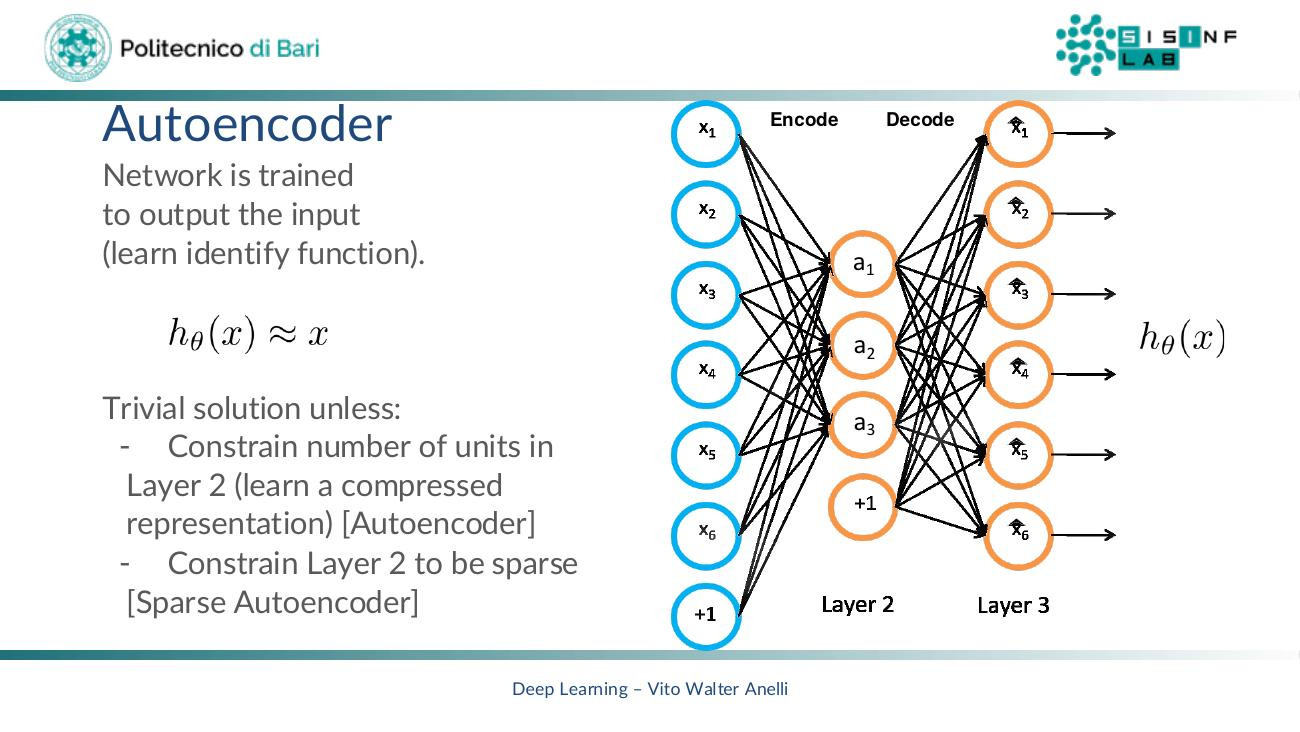
\includegraphics[width=0.82\linewidth]{figures/cf10_ae_architecture.jpg}
  \caption{Architettura di un autoencoder con 6 neuroni di input, 3 unità
           latenti $a_1, a_2, a_3$ (Layer~2) e 6 neuroni di output (Layer~3).
           La rete apprende la funzione $h_\theta(\mathbf{x}) \approx
           \mathbf{x}$ attraverso il collo di bottiglia.}
  \label{fig:ae_architecture}
\end{figure}

\subsection{Sparse Autoencoder}
\label{subsec:sparse-ae}

Nello \textbf{sparse autoencoder} la dimensionalità del collo di bottiglia
può anche essere maggiore di quella dell'input ($k > d$,
\emph{overcomplete}), ma le attivazioni latenti vengono penalizzate con un
termine L1 che le forza a essere sparse:

\begin{equation}
  \mathcal{L}_{\text{sparse}} = \underbrace{\|h_\theta(\mathbf{x}) -
    \mathbf{x}\|^2}_{\text{errore di ricostruzione}}
    + \lambda \underbrace{\sum_{i} |a_i|}_{\text{termine L1 di sparsità}},
  \label{eq:sparse-ae-loss}
\end{equation}

dove $a_i$ è l'attivazione dell'$i$-esima unità latente. Il vincolo
di sparsità induce la rete a usare solo poche unità attive per ogni
esempio, producendo una rappresentazione distribuita e interpretabile.
Questa formulazione è strettamente collegata alla \emph{dictionary
learning} e ai metodi di codifica sparsa \citep{bishop2024}.

%------------------------------------------------------------
\section{Deep Autoencoder}
\label{sec:deep-ae}

\subsection{Stacking di Autoencoder}
\label{subsec:stacking}

La profondità può essere aumentata impilando più coppie encoder-decoder.
Ogni livello impara una rappresentazione sempre più astratta dell'input;
i pesi dei livelli di decodifica sono tipicamente condivisi (o trasposti)
rispetto ai livelli di codifica (\emph{tied weights}):

\begin{equation}
  W_{\text{dec},\ell} = W_{\text{enc},\ell}^T.
  \label{eq:tied-weights}
\end{equation}

\begin{figure}[H]
  \centering
  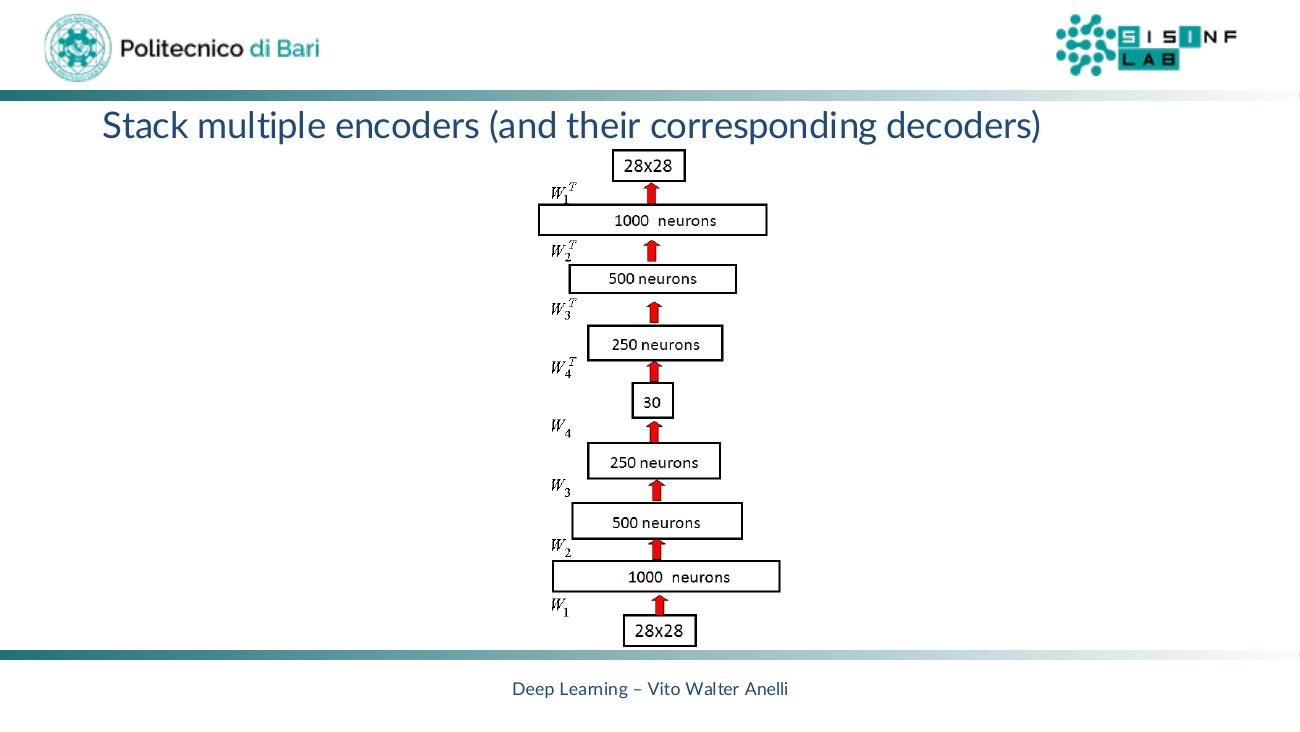
\includegraphics[width=0.55\linewidth]{figures/cf10_deep_ae_stacked.jpg}
  \caption{Deep autoencoder per immagini $28\times28$ (MNIST): il percorso
           di codifica comprime $784 \to 1000 \to 500 \to 250 \to 30$
           neuroni; il percorso di decodifica (con pesi $W_i^T$) ricostruisce
           simmetricamente fino alla dimensione originale.}
  \label{fig:deep_ae}
\end{figure}

\subsection{Confronto con la PCA}
\label{subsec:ae-vs-pca}

Un autoencoder lineare a un livello nascosto apprende esattamente lo
stesso sottospazio della \textbf{PCA}: il collo di bottiglia proietta
i dati sulle $k$ componenti principali a maggiore varianza. Un autoencoder
\emph{non lineare} (con funzioni di attivazione) apprende una varietà
non lineare, catturando strutture più complesse.

\begin{figure}[H]
  \centering
  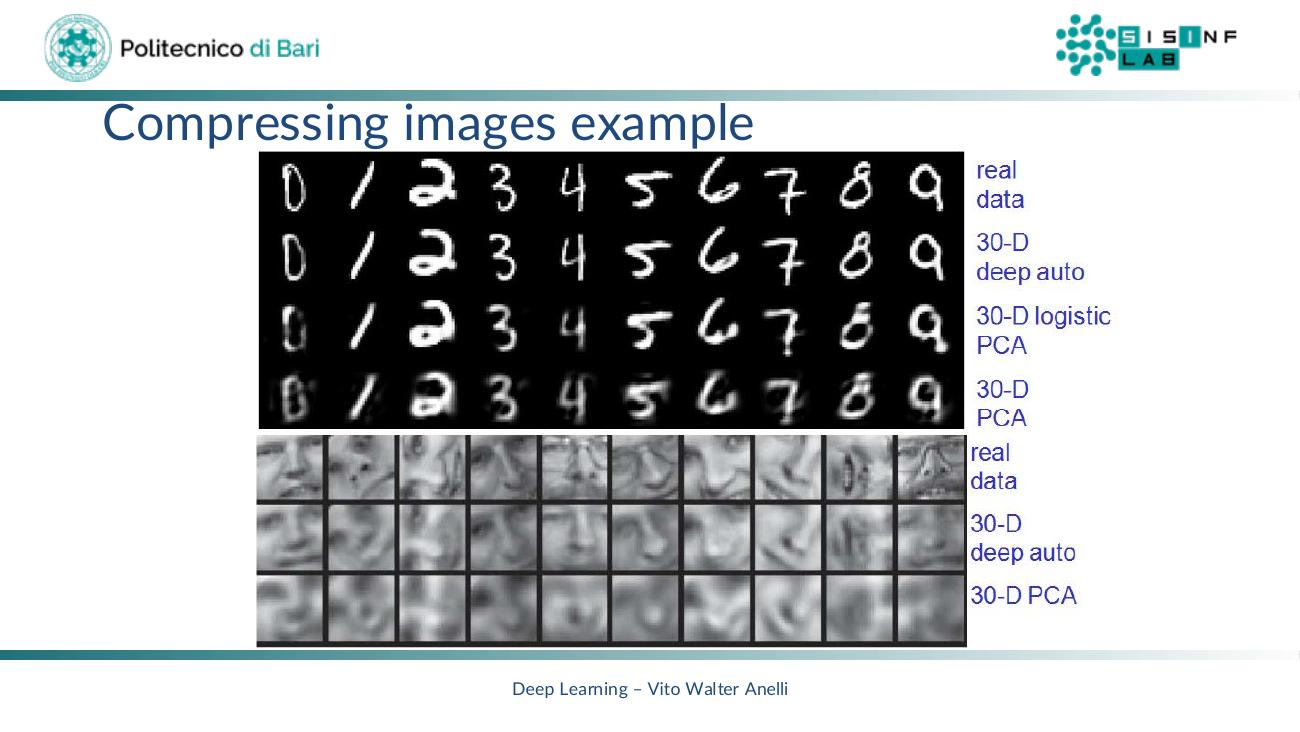
\includegraphics[width=0.82\linewidth]{figures/cf10_ae_compression_mnist.jpg}
  \caption{Compressione a 30 dimensioni su MNIST (sopra) e su volti
           (sotto). Il deep autoencoder (riga 2) preserva dettagli fini che
           la PCA lineare a 30 componenti (riga~4) non riesce a catturare,
           confermando la superiorità delle rappresentazioni non lineari.}
  \label{fig:ae_compression}
\end{figure}

%------------------------------------------------------------
\section{U-Net}
\label{sec:unet}

\subsection{Segmentazione Semantica}
\label{subsec:semantic-segmentation}

La \textbf{segmentazione semantica} è il compito di assegnare una classe
a ogni singolo pixel di un'immagine. I modelli sono addestrati usando
\emph{mappe di segmentazione} come target: per ogni immagine si dispone
di una mappa binaria che distingue i pixel di interesse (es.\ cellule
biologiche) da quelli di sfondo. La perdita tipica per questa formulazione
è la \textbf{cross-entropy binaria} pixel-per-pixel o la
\textbf{Dice loss}, che massimizza la sovrapposizione tra maschera
predetta e maschera vera.

\subsection{Architettura U-Net}
\label{subsec:unet-architecture}

La \textbf{U-Net} \citep{ronneberger2015unet} è un autoencoder
convoluzionale progettato per la segmentazione semantica, originariamente
concepita per immagini medicali. La struttura simmetrica a forma di U
comprende tre componenti:

\begin{description}
  \item[Percorso contrattivo (Encoder)] Sequenze di blocchi convoluzionali
        seguiti da max-pooling; riduce progressivamente la risoluzione
        spaziale aumentando il numero di feature map.
  \item[Percorso espansivo (Decoder)] Blocchi di deconvoluzione
        (convoluzione trasposta) che ripristinano la risoluzione spaziale,
        alternati a convoluzioni standard.
  \item[Skip connections] Connessioni dirette che concatenano le feature
        map del percorso contrattivo al livello corrispondente del percorso
        espansivo.
\end{description}

\begin{figure}[H]
  \centering
  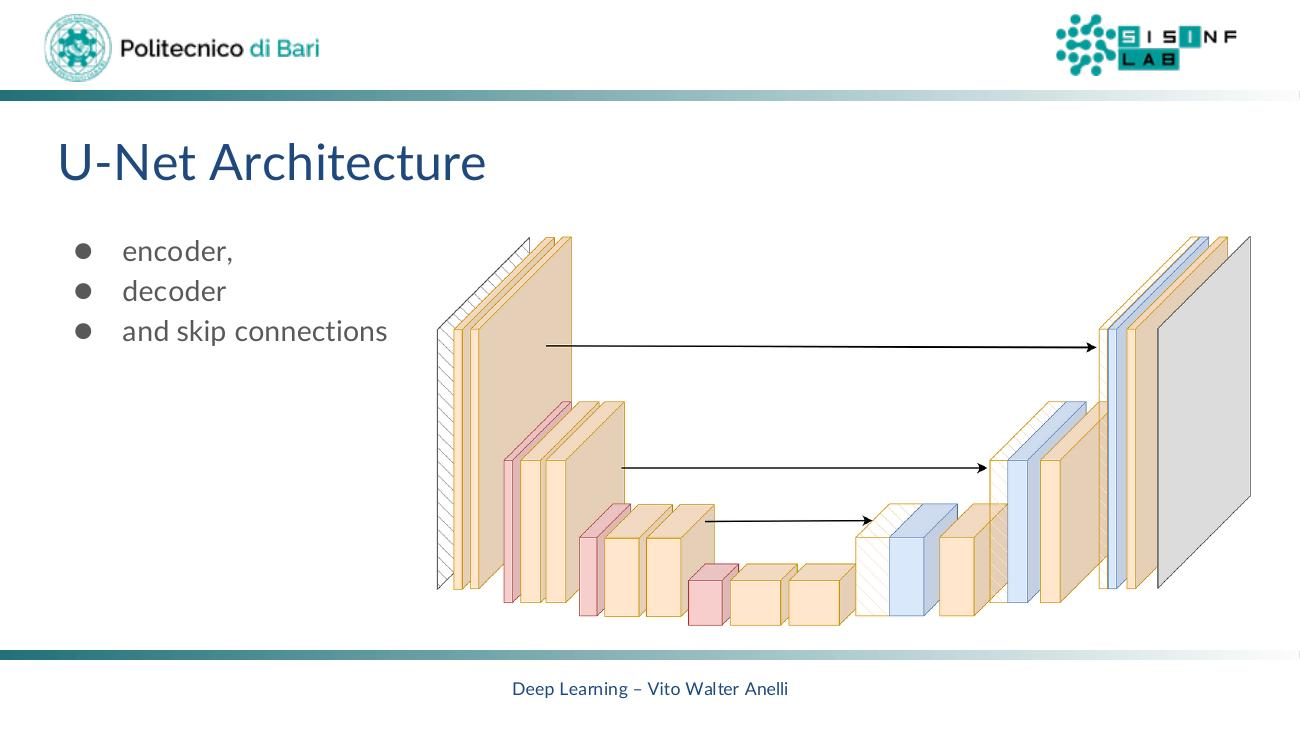
\includegraphics[width=0.82\linewidth]{figures/cf10_unet_architecture.jpg}
  \caption{Architettura U-Net: la forma a U è evidente dalla progressiva
           riduzione spaziale nel percorso di sinistra (encoder) e dalla
           riespansione nel percorso di destra (decoder). Le frecce
           orizzontali rappresentano le skip connections.}
  \label{fig:unet_arch}
\end{figure}

\subsection{Skip Connections}
\label{subsec:skip-connections}

Le skip connections sono la differenza architettonica cruciale rispetto
a un autoencoder classico, nel quale encoder e decoder devono essere
strettamente separati (altrimenti la compressione non avrebbe senso).
Nella U-Net questa restrizione non esiste: l'output è una mappa di
segmentazione della \emph{stessa risoluzione} dell'input, non una
ricostruzione.

Ogni skip connection concatena l'ultimo feature map del blocco
convoluzionale $k$ con l'output del blocco deconvoluzionale
corrispondente, fornendo due tipi di informazione complementari:

\begin{itemize}
  \item \textbf{Estrazione di feature}: le feature ad alto livello
        apprese nel percorso espansivo.
  \item \textbf{Localizzazione}: la posizione spaziale delle feature
        estratte dal corrispondente livello convoluzionale dell'encoder.
\end{itemize}

\begin{figure}[H]
  \centering
  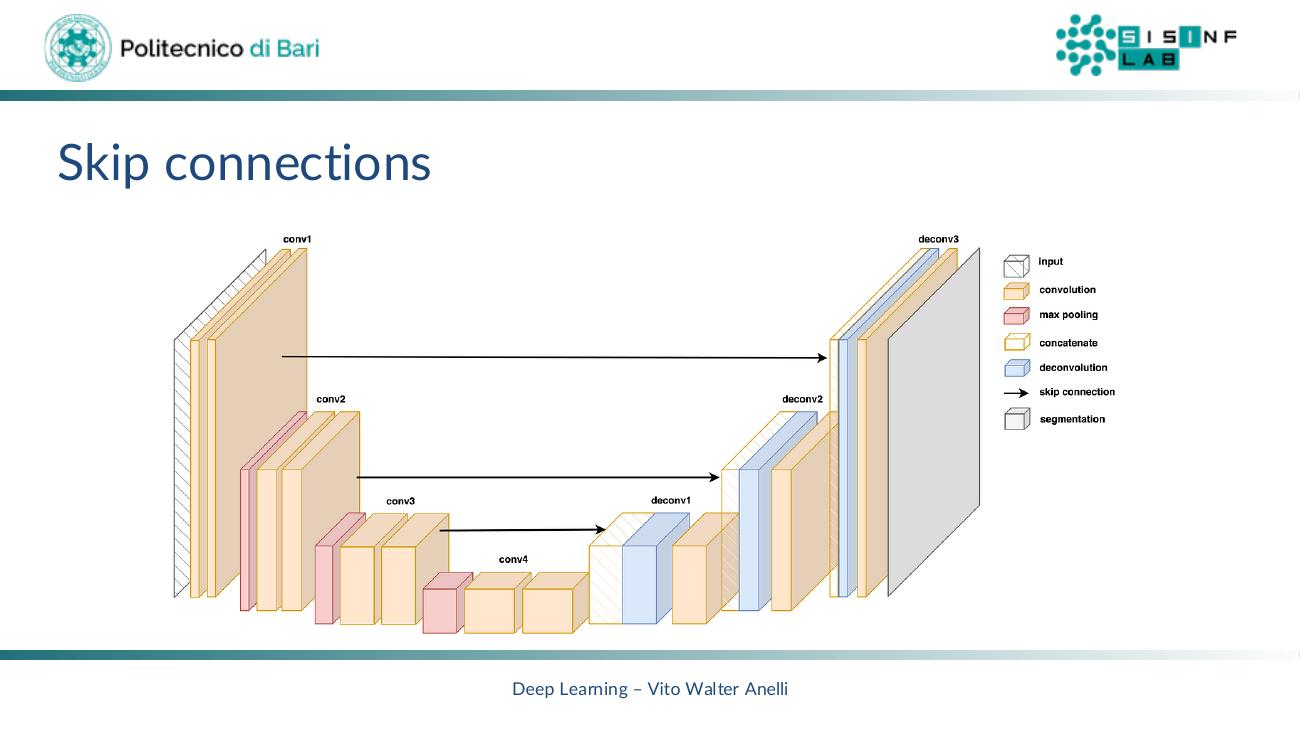
\includegraphics[width=0.82\linewidth]{figures/cf10_unet_skip_connections.jpg}
  \caption{Skip connections nella U-Net: ogni freccia orizzontale
           (conv\,1$\to$deconv\,3, conv\,2$\to$deconv\,2, conv\,3$\to$deconv\,1)
           concatena la mappa del livello convoluzionale con quella del
           corrispondente livello deconvoluzionale, combinando localizzazione
           e semantica.}
  \label{fig:unet_skip}
\end{figure}

\subsection{Deconvoluzione e Upsampling}
\label{subsec:deconvolution}

Il percorso espansivo utilizza \textbf{convoluzione trasposta}
(\emph{deconvolution} o \emph{transposed convolution}) per aumentare
la risoluzione spaziale in modo apprendibile, a differenza del
max-pooling che usa una regola fissa. In Keras/TensorFlow:

\begin{lstlisting}[language=Python, caption={Blocco espansivo U-Net in
  Keras.}, label={lst:unet-block}]
deconv = Conv2DTranspose(filters, (3,3),
                         strides=(2,2), padding="same")(prev)
uconv  = concatenate([deconv, skip_conv])   # skip connection
uconv  = Dropout(0.5)(uconv)
uconv  = Conv2D(filters, (3,3), activation="relu",
                padding="same")(uconv)
uconv  = Conv2D(filters, (3,3), activation="relu",
                padding="same")(uconv)
\end{lstlisting}

\paragraph{Layer di output.}
Il layer finale è una convoluzione $1\times1$ con attivazione sigmoide
che mappa ogni pixel a una probabilità di appartenenza alla classe
target. Nella U-Net \emph{non sono presenti layer fully-connected}:
l'intera rete è \emph{fully convolutional}, il che la rende applicabile
a immagini di dimensioni arbitrarie.

\begin{lstlisting}[language=Python, caption={Layer di output U-Net.},
  label={lst:unet-output}]
output = Conv2D(1, (1,1), padding="same",
                activation="sigmoid")(uconv1)
\end{lstlisting}

%------------------------------------------------------------
\section{Variational Autoencoder (VAE)}
\label{sec:vae}

\subsection{Limitazioni dell'Autoencoder Classico}
\label{subsec:ae-limitations}

Nell'autoencoder classico il collo di bottiglia mappa ogni input in un
\emph{punto} dello spazio latente. Campionare un punto arbitrario da
tale spazio e decodificarlo non produce necessariamente output
semanticamente significativi: lo spazio latente non è strutturato in
modo da garantire \emph{continuità} (punti vicini $\Rightarrow$ output
simili) né \emph{completezza} (ogni punto è decodificabile
in modo sensato). Il VAE risolve questi limiti imponendo una
\textbf{regolarizzazione probabilistica} sullo spazio latente.

\subsection{Confronto AE vs VAE: Flusso Computazionale}
\label{subsec:ae-vs-vae}

\begin{figure}[H]
  \centering
  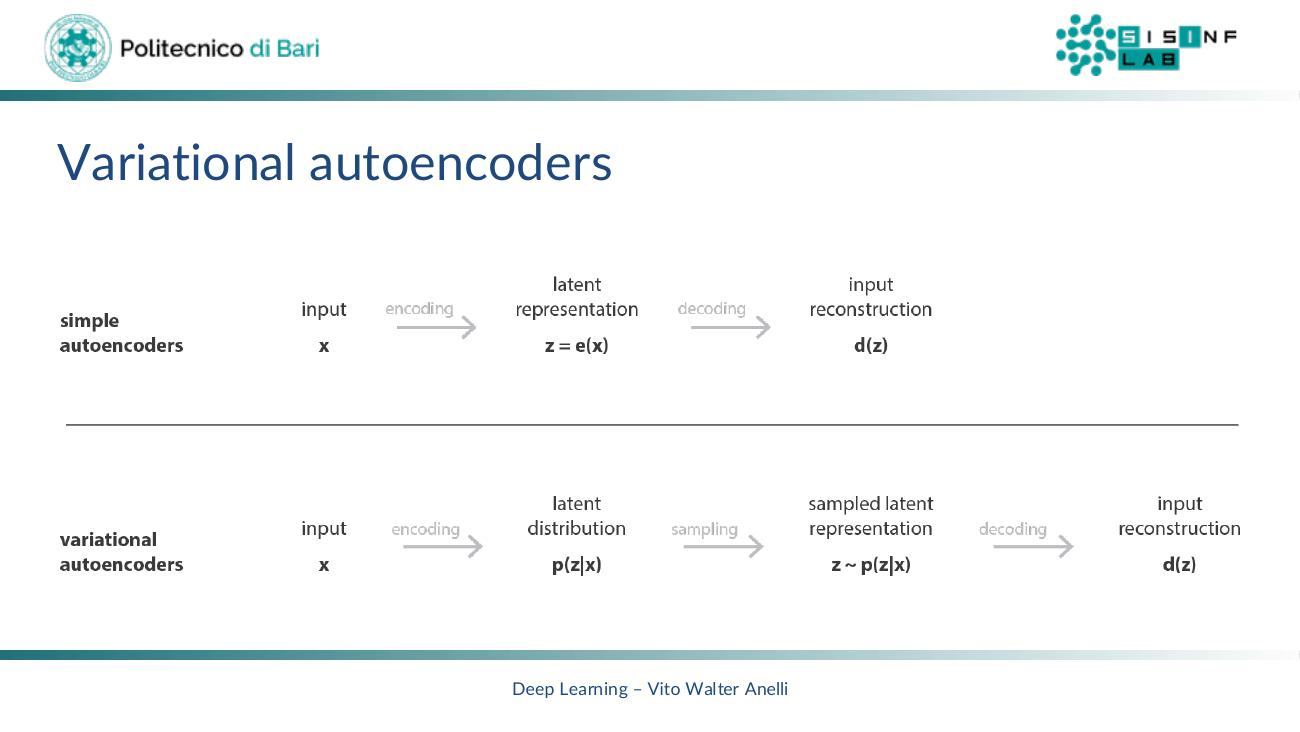
\includegraphics[width=0.82\linewidth]{figures/cf10_ae_vs_vae_flow.jpg}
  \caption{Confronto tra autoencoder classico (sopra) e variazionale
           (sotto). Nell'AE classico l'encoder produce un punto
           $\mathbf{z} = e(\mathbf{x})$; nel VAE produce una
           \emph{distribuzione} $p(\mathbf{z}|\mathbf{x})$, da cui viene
           campionato $\mathbf{z}$ prima della decodifica.}
  \label{fig:ae_vs_vae}
\end{figure}

\subsection{Modello Probabilistico}
\label{subsec:vae-probabilistic}

Il VAE \citep{kingma2014vae} adotta una prospettiva generativa. Si
definiscono due variabili:

\begin{itemize}
  \item $\mathbf{x}$: i dati osservati.
  \item $\mathbf{z}$: variabile latente \emph{non osservata} (rappresentazione
        compressa).
\end{itemize}

Il processo generativo assume:

\begin{align}
  p(\mathbf{z}) &\equiv \mathcal{N}(\mathbf{0}, \mathbf{I})
    \quad \text{(prior standard gaussiana)},
  \label{eq:vae-prior} \\
  p(\mathbf{x}|\mathbf{z}) &\equiv \mathcal{N}(f(\mathbf{z}),\, c\mathbf{I})
    \quad f \in F,\; c > 0
  \label{eq:vae-likelihood}
\end{align}

dove $f$ è la funzione \textbf{decoder} (una rete neurale) e $c$ è un
iperparametro di scala della varianza. Si ridefiniscono encoder e decoder
in termini probabilistici:

\begin{description}
  \item[Decoder probabilistico] $p(\mathbf{x}|\mathbf{z})$: distribuzione
        della variabile decodificata dato il codice.
  \item[Encoder probabilistico] $p(\mathbf{z}|\mathbf{x})$: distribuzione
        della variabile latente dato l'input (posteriore di Bayes).
\end{description}

\paragraph{Il teorema di Bayes nel VAE.}
Per il teorema di Bayes:

\begin{equation}
  p(\mathbf{z}|\mathbf{x}) = \frac{p(\mathbf{x}|\mathbf{z})\,p(\mathbf{z})}{p(\mathbf{x})}
  = \frac{p(\mathbf{x}|\mathbf{z})\,p(\mathbf{z})}{\displaystyle\int p(\mathbf{x}|\mathbf{u})\,p(\mathbf{u})\,d\mathbf{u}}.
  \label{eq:bayes-vae}
\end{equation}

L'integrale al denominatore è \textbf{intrattabile} nella maggior parte
dei casi (richiede l'integrazione su tutto lo spazio latente), pertanto
si ricorre all'inferenza variazionale.

\subsection{Inferenza Variazionale}
\label{subsec:variational-inference}

L'\textbf{inferenza variazionale} (VI) approssima la posteriore
$p(\mathbf{z}|\mathbf{x})$, intrattabile, con una distribuzione più semplice
$q_\mathbf{x}(\mathbf{z})$ parametrizzata da una famiglia di gaussiane:

\begin{equation}
  q_\mathbf{x}(\mathbf{z}) \equiv \mathcal{N}(g(\mathbf{x}),\, h(\mathbf{x})),
  \quad g \in G,\; h \in H,
  \label{eq:vi-approx}
\end{equation}

dove $g$ e $h$ (le funzioni che producono media e varianza) sono
implementate come rami dell'encoder. La coppia ottimale $(g^*, h^*)$
minimizza la \textbf{divergenza di Kullback-Leibler}:

\begin{align}
  (g^*, h^*) &= \operatorname*{arg\,min}_{(g,h) \in G \times H}
    \mathrm{KL}\!\left(q_\mathbf{x}(\mathbf{z})\,\|\,p(\mathbf{z}|\mathbf{x})\right)
  \notag \\
  &= \operatorname*{arg\,max}_{(g,h) \in G \times H}
    \left(\mathbb{E}_{\mathbf{z} \sim q_\mathbf{x}}
      \!\left[\log p(\mathbf{x}|\mathbf{z})\right]
    - \mathrm{KL}\!\left(q_\mathbf{x}(\mathbf{z})\,\|\,p(\mathbf{z})\right)
    \right).
  \label{eq:vi-objective}
\end{align}

Il secondo membro della \eqref{eq:vi-objective} è chiamato
\textbf{Evidence Lower Bound} (ELBO).

\subsection{Funzione di Loss del VAE}
\label{subsec:vae-loss}

Incorporando anche la scelta del decoder $f$, l'obiettivo completo del
VAE è:

\begin{equation}
  (f^*, g^*, h^*) = \operatorname*{arg\,max}_{(f,g,h) \in F \times G \times H}
    \left(\mathbb{E}_{\mathbf{z} \sim q_\mathbf{x}}\!\left[
      -\frac{\|\mathbf{x} - f(\mathbf{z})\|^2}{2c}
    \right]
    - \mathrm{KL}\!\left(q_\mathbf{x}(\mathbf{z}),\, p(\mathbf{z})\right)
    \right).
  \label{eq:vae-full-objective}
\end{equation}

Equivalentemente, minimizzando il negativo dell'ELBO, la loss del VAE è:

\begin{equation}
  \mathcal{L}_{\text{VAE}} =
    \underbrace{C\,\|\mathbf{x} - f(\mathbf{z})\|^2}_{\text{errore di ricostruzione}}
    + \underbrace{\mathrm{KL}\!\left[\mathcal{N}(\boldsymbol{\mu}_\mathbf{x},
    \boldsymbol{\sigma}_\mathbf{x}),\, \mathcal{N}(\mathbf{0}, \mathbf{I})\right]}_{\text{termine di regolarizzazione}},
  \label{eq:vae-loss}
\end{equation}

dove $\boldsymbol{\mu}_\mathbf{x} = g(\mathbf{x})$ e
$\boldsymbol{\sigma}_\mathbf{x} = h(\mathbf{x})$ sono i parametri
della distribuzione latente prodotti dall'encoder. La KL-divergenza tra
due gaussiane ha forma chiusa:

\begin{equation}
  \mathrm{KL}\!\left[\mathcal{N}(\boldsymbol{\mu}, \boldsymbol{\sigma}^2\mathbf{I}),\,
    \mathcal{N}(\mathbf{0}, \mathbf{I})\right]
  = \frac{1}{2}\sum_{j}\!\left(\sigma_j^2 + \mu_j^2 - 1 - \log\sigma_j^2\right).
  \label{eq:kl-gaussian}
\end{equation}

\begin{figure}[H]
  \centering
  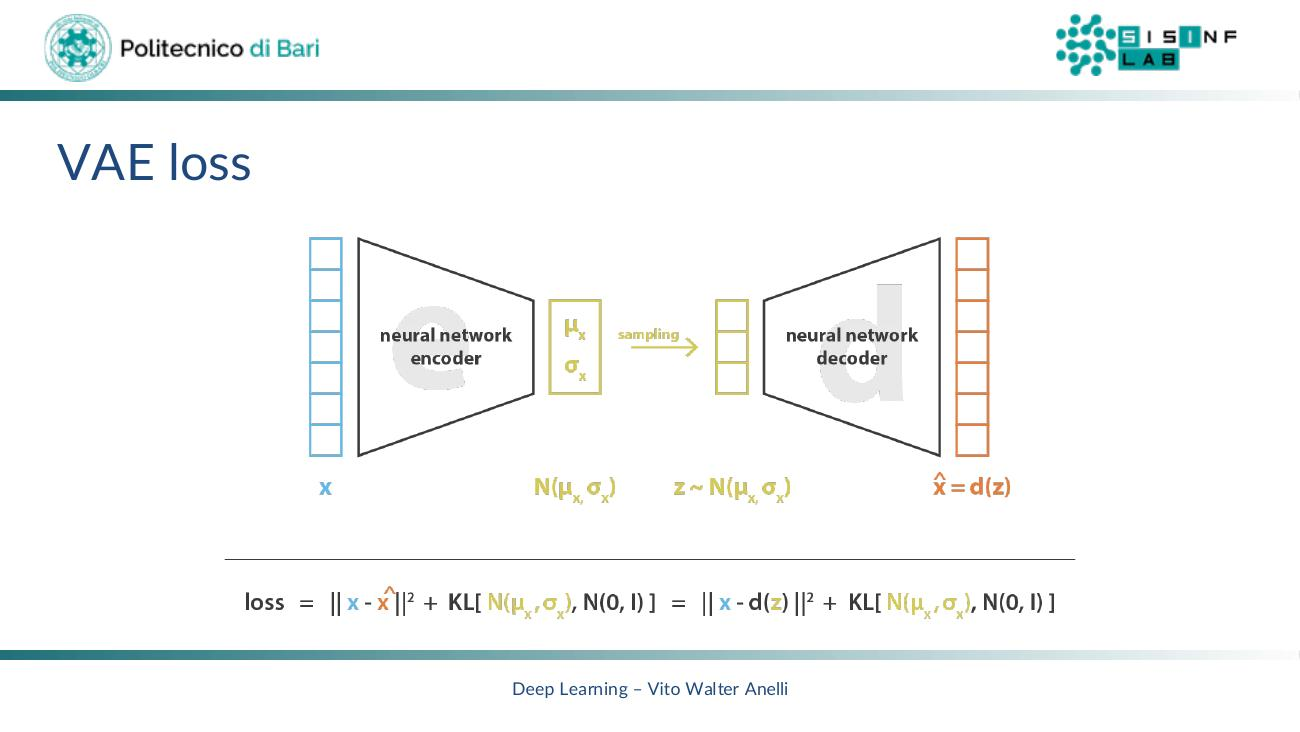
\includegraphics[width=0.82\linewidth]{figures/cf10_vae_loss_diagram.jpg}
  \caption{Schema della loss del VAE. L'encoder produce
           $(\boldsymbol{\mu}_\mathbf{x}, \boldsymbol{\sigma}_\mathbf{x})$;
           un punto $\mathbf{z} \sim \mathcal{N}(\boldsymbol{\mu}_\mathbf{x},
           \boldsymbol{\sigma}_\mathbf{x})$ viene decodificato in
           $\hat{\mathbf{x}} = d(\mathbf{z})$. La loss combina
           errore di ricostruzione e KL-divergenza.}
  \label{fig:vae_loss}
\end{figure}

\subsection{Proprietà dello Spazio Latente Regolarizzato}
\label{subsec:vae-latent-space}

Le due proprietà fondamentali che la regolarizzazione KL impone allo
spazio latente sono:

\begin{description}
  \item[Continuità] Punti vicini nello spazio latente producono output
        simili una volta decodificati.
  \item[Completezza] Qualsiasi punto campionato dalla prior
        $p(\mathbf{z}) = \mathcal{N}(\mathbf{0},\mathbf{I})$ produce un
        output semanticamente significativo.
\end{description}

Senza regolarizzazione, l'encoder potrebbe imparare distribuzioni con
varianza nulla (riducendosi a un autoencoder classico) o con medie molto
distanti tra loro, rendendo lo spazio latente discontinuo e privo di
significato generativo.

\begin{figure}[H]
  \centering
  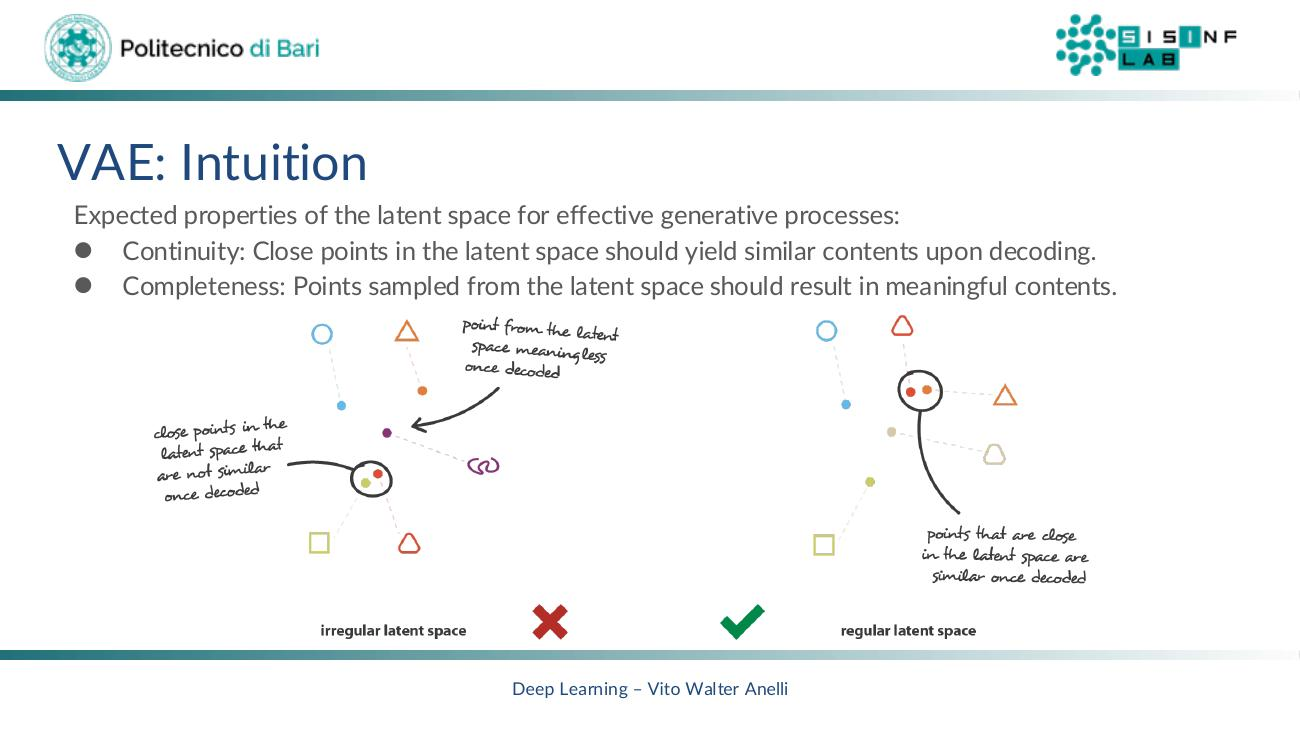
\includegraphics[width=0.82\linewidth]{figures/cf10_vae_latent_space_intuition.jpg}
  \caption{Confronto tra spazio latente irregolare (sinistra, autoencoder
           senza regolarizzazione: punti vicini non simili, regioni vuote)
           e spazio latente regolare (destra, VAE: distribuzioni continue
           e sovrapposte, proprietà di continuità e completezza
           garantite).}
  \label{fig:vae_latent}
\end{figure}

\subsection{Il Reparametrization Trick}
\label{subsec:reparam-trick}

Il campionamento $\mathbf{z} \sim \mathcal{N}(\boldsymbol{\mu}_\mathbf{x},
\boldsymbol{\sigma}_\mathbf{x})$ è un'operazione \emph{stocastica} non
differenziabile; i gradienti non possono fluire attraverso di essa verso i
parametri dell'encoder. Il \textbf{reparametrization trick}
\citep{kingma2014vae} risolve il problema spostando la stocasticità su
una variabile ausiliaria $\boldsymbol{\zeta}$ indipendente dai parametri:

\begin{equation}
  \boldsymbol{\zeta} \sim \mathcal{N}(\mathbf{0}, \mathbf{I}),
  \qquad
  \mathbf{z} = \boldsymbol{\sigma}_\mathbf{x} \odot \boldsymbol{\zeta}
             + \boldsymbol{\mu}_\mathbf{x}.
  \label{eq:reparam}
\end{equation}

Il grafo computazionale risultante è differenziabile rispetto a
$\boldsymbol{\mu}_\mathbf{x}$ e $\boldsymbol{\sigma}_\mathbf{x}$, poiché
il campionamento avviene su $\boldsymbol{\zeta}$, che non dipende dai
parametri della rete.

\begin{figure}[H]
  \centering
  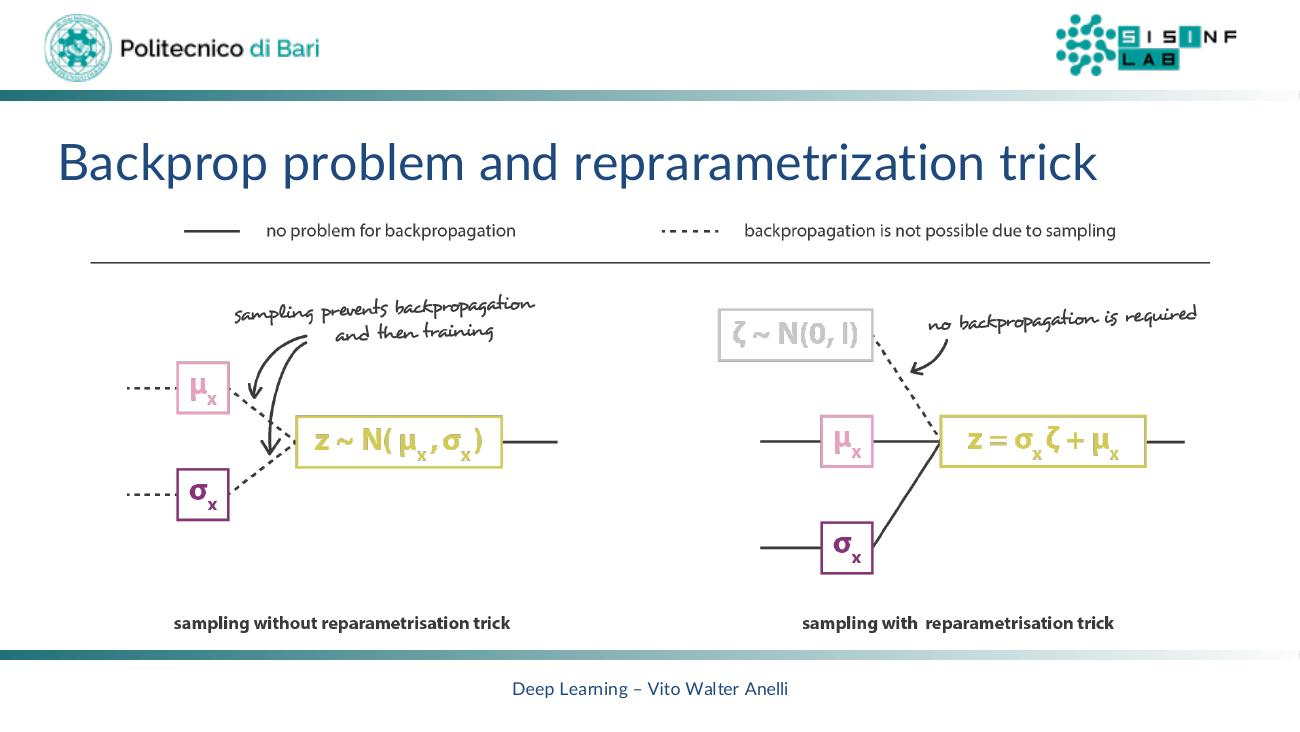
\includegraphics[width=0.82\linewidth]{figures/cf10_vae_reparam_trick.jpg}
  \caption{Reparametrization trick. Sinistra: il campionamento diretto
           $\mathbf{z} \sim \mathcal{N}(\boldsymbol{\mu}_\mathbf{x},
           \boldsymbol{\sigma}_\mathbf{x})$ blocca la backpropagation
           (linee tratteggiate). Destra: con il trick,
           $\boldsymbol{\zeta} \sim \mathcal{N}(\mathbf{0},\mathbf{I})$
           è esterno al grafo, e la trasformazione
           $\mathbf{z} = \boldsymbol{\sigma}_\mathbf{x}\boldsymbol{\zeta}
           + \boldsymbol{\mu}_\mathbf{x}$ è differenziabile (linee
           continue).}
  \label{fig:reparam}
\end{figure}

\subsection{Schema Completo del VAE}
\label{subsec:vae-complete}

\begin{figure}[H]
  \centering
  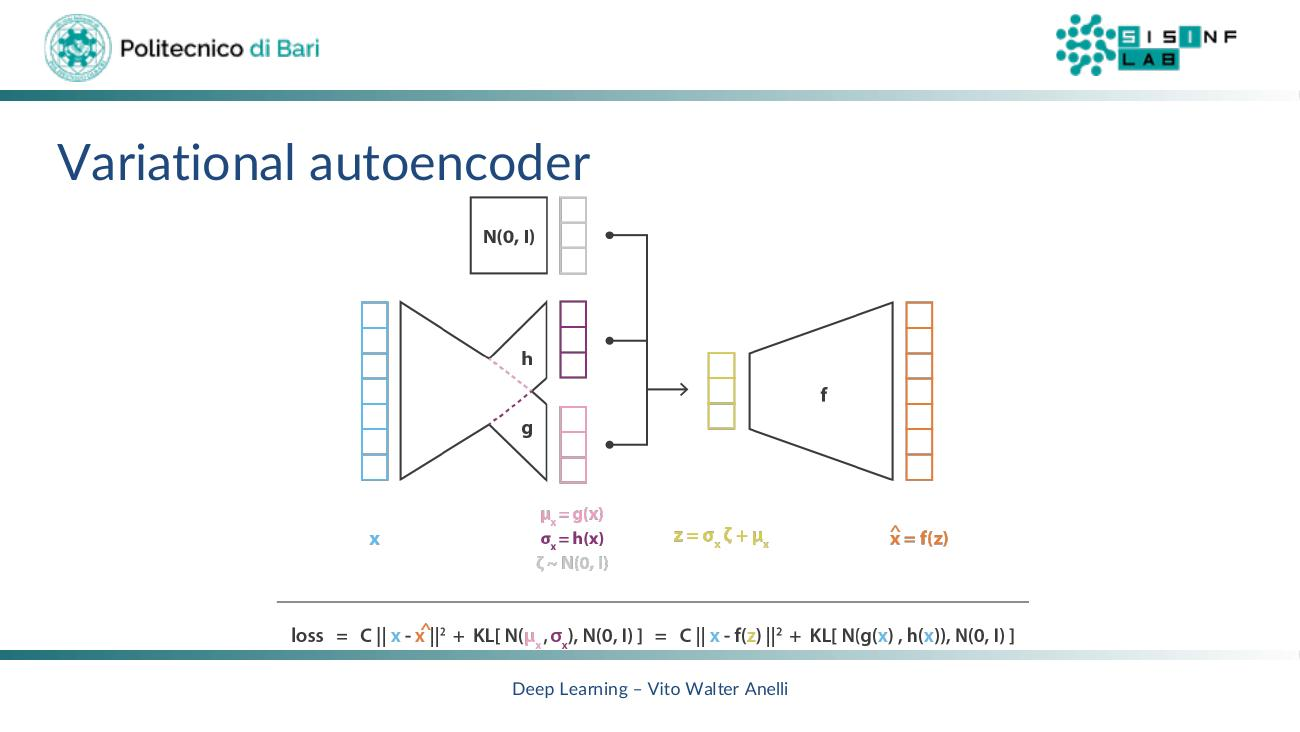
\includegraphics[width=0.88\linewidth]{figures/cf10_vae_full_diagram.jpg}
  \caption{Schema completo del VAE con reparametrization trick. L'encoder
           produce $\boldsymbol{\mu}_\mathbf{x} = g(\mathbf{x})$ e
           $\boldsymbol{\sigma}_\mathbf{x} = h(\mathbf{x})$; il campionamento
           è realizzato tramite $\mathbf{z} = \boldsymbol{\sigma}_\mathbf{x}
           \boldsymbol{\zeta} + \boldsymbol{\mu}_\mathbf{x}$ con
           $\boldsymbol{\zeta} \sim \mathcal{N}(\mathbf{0},\mathbf{I})$;
           il decoder restituisce $\hat{\mathbf{x}} = f(\mathbf{z})$. La loss
           è la somma di errore di ricostruzione e KL-divergenza.}
  \label{fig:vae_full}
\end{figure}

\paragraph{Implementazione in PyTorch.}

\begin{lstlisting}[language=Python, caption={VAE: encoder, reparametrization
  e loss in PyTorch.}, label={lst:vae-pytorch}]
import torch
import torch.nn as nn
import torch.nn.functional as F

class VAE(nn.Module):
    def __init__(self, d_in, d_h, d_z):
        super().__init__()
        # Encoder: produce mu e log-varianza
        self.fc1    = nn.Linear(d_in, d_h)
        self.fc_mu  = nn.Linear(d_h, d_z)
        self.fc_log = nn.Linear(d_h, d_z)
        # Decoder
        self.fc3    = nn.Linear(d_z, d_h)
        self.fc4    = nn.Linear(d_h, d_in)

    def encode(self, x):
        h = F.relu(self.fc1(x))
        return self.fc_mu(h), self.fc_log(h)

    def reparametrize(self, mu, log_var):
        std = torch.exp(0.5 * log_var)
        zeta = torch.randn_like(std)   # N(0,I)
        return mu + std * zeta         # eq. (10.13)

    def decode(self, z):
        h = F.relu(self.fc3(z))
        return torch.sigmoid(self.fc4(h))

    def forward(self, x):
        mu, log_var = self.encode(x)
        z = self.reparametrize(mu, log_var)
        x_hat = self.decode(z)
        return x_hat, mu, log_var

def vae_loss(x_hat, x, mu, log_var):
    rec = F.mse_loss(x_hat, x, reduction="sum")
    kl  = -0.5 * torch.sum(
              1 + log_var - mu.pow(2) - log_var.exp())
    return rec + kl
\end{lstlisting}

%------------------------------------------------------------
\section{Confronto e Riepilogo}
\label{sec:ae-summary}

\begin{table}[H]
  \centering
  \caption{Confronto tra le varianti di autoencoder trattate.}
  \label{tab:ae-comparison}
  \small
  \begin{tabular}{lllll}
    \toprule
    \textbf{Modello} & \textbf{Vincolo} & \textbf{Spazio latente}
      & \textbf{Generativo} & \textbf{Applicazione tipica} \\
    \midrule
    AE classico & $k < d$ & Punto & No & Compressione, pre-training \\
    Sparse AE   & $\ell_1$ su $\mathbf{a}$ & Punto sparso & No &
      Feature learning \\
    Deep AE     & Più livelli & Punto profondo & No &
      Compressione non lineare \\
    U-Net       & Skip connections & --- & No &
      Segmentazione semantica \\
    VAE         & KL$(\cdot\|\mathcal{N}(\mathbf{0},\mathbf{I}))$ &
      Distribuzione & Sì & Generazione, interpolazione \\
    \bottomrule
  \end{tabular}
\end{table}

\paragraph{Linee guida pratiche.}
\begin{enumerate}
  \item Per \textbf{compressione} o \textbf{riduzione dimensionale}:
        usare un deep autoencoder con tied weights; la dimensione del
        collo di bottiglia è un iperparametro da cercare tramite
        validation.
  \item Per \textbf{feature learning} non supervisionato: preferire lo
        sparse autoencoder (o un denoising autoencoder, che aggiunge
        rumore all'input e lo richiede pulito all'uscita).
  \item Per \textbf{segmentazione semantica pixel-per-pixel}: usare la
        U-Net con skip connections; la scelta della profondità ($n$ livelli
        di pooling) dipende dalla risoluzione dell'immagine.
  \item Per \textbf{generazione} e \textbf{interpolazione nello spazio
        latente}: usare un VAE; il bilanciamento tra termine di
        ricostruzione e termine KL (tramite un iperparametro $\beta$,
        come nel $\beta$-VAE) controlla il trade-off tra qualità
        ricostruttiva e regolarità dello spazio latente.
  \item Ricordare il reparametrization trick: senza di esso la
        backpropagation non attraversa il nodo di campionamento e
        l'addestramento del VAE non converge.
\end{enumerate}

Come sottolinea \citet{bishop2024}, gli autoencoder rappresentano un
paradigma fondamentale dell'apprendimento non supervisionato: la
successione AE $\to$ Sparse AE $\to$ Denoising AE $\to$ VAE traccia
un percorso verso modelli generativi sempre più strutturati, che
costituisce la base concettuale dei modelli di diffusione moderni.